%% Tipo de documento %%
\documentclass[aspectratio=169]{beamer}

%% Paquetes %%
\usepackage{adjustbox}
\usepackage{amsmath}
\usepackage{array}
\usepackage{booktabs}
\usepackage{geometry}
\usepackage{graphicx}
\usepackage{natbib}
\usepackage[utf8]{inputenc}
\usepackage{multirow}
\usepackage[T1]{fontenc}
\usepackage[spanish]{babel}
\usepackage{tikz}
\usepackage{relsize}
\usetikzlibrary{positioning,tikzmark,fit,arrows.meta,trees,decorations.pathreplacing,shapes.geometric, fit, calc}
\usepackage{numprint}
\newtheorem{ejemplo}{Ejemplo}[section]
\setbeamertemplate{theorems}[numbered]

%% Configuración de los número de página %%
\setbeamertemplate{footline}[frame number]
\setbeamertemplate{caption}[numbered]

%% Imagen de fondo en la primera dispositiva %%
\setbeamertemplate{background canvas}{
  
\includegraphics[width=\paperwidth, height=\paperheight]{front.jpg}
}

%% Ubicación del título y subtitulo de cada dispositiva %%
\setbeamertemplate{frametitle}{
	\vspace{1cm}
	\textcolor{blue}{\bf \insertframetitle}\\
	\normalsize
	\textcolor{black}{\bf \insertframesubtitle}
}

%% Información de la primera dispositiva %%
\title[Doctorado en Inteligencia Artificial]{\textcolor{white}{\bf{ Datos normativos para la prueba de aprendizaje y memoria (TAMV-I) en niños latinoamericanos y españoles: un enfoque basado en la teoría de respuesta al ítem y modelos lineales mixtos}}}
%\subtitle{\textcolor{white}{\bf{Nodo Universidad Simón Bolívar}}}
\author{\textcolor{white}{\bf{Dr. Erick Orozco-Acosta}}}
%\institute{\textcolor{white}{\bf{Facultad de Ciencias de la Salud}}}
\date{\textcolor{white}{\bf{Barranquilla 2026}}}

%%%%%%%%%%%%%%%%%%%%%%%%%%%%%%%%%%%%%%%%%%%%%%%%%%%%%%%%%%%%%%%%%
%%%%%%%%%%%%%%%%%%%%%%%%%%% Inicio del documento %%%%%%%%%%%%%%%%%%%%%%%%%%%
%%%%%%%%%%%%%%%%%%%%%%%%%%%%%%%%%%%%%%%%%%%%%%%%%%%%%%%%%%%%%%%%%

\begin{document}
%------------------------------------------------
\begin{frame}
	\titlepage
\end{frame}
%------------------------------------------------
%% Imagen de fondo regular %%
\setbeamertemplate{background canvas}{
	
\includegraphics[width=\paperwidth,height=\paperheight]{contenido.jpg}
}
%------------------------------------------------
\begin{frame}{Colaboración Internacional }
	\begin{columns}[T]
		
		% Columna izquierda
		\begin{column}{0.5\textwidth}
			\small
			
			\textbf{Institución anfitriona}
			
			\begin{itemize}
				\item Universidad Pública de Navarra
				\item Grupo de investigación NeO Neurozientziak eta Ongizatea
			\end{itemize}
			
			\vspace{0.2cm}
			
			\textbf{Actividades desarrolladas}
			
			\begin{itemize}
				\item Evaluación y Rehabilitación Neuropsicológica
				\item Psicometría y Métodos Cuantitativos
				\item Daño Cerebral
				\item Neurociencia cognitiva
			\end{itemize}
			
		\end{column}
		
		% Columna derecha
		\begin{column}{0.55\textwidth}
			\vspace{-2.3cm}
			\centering
			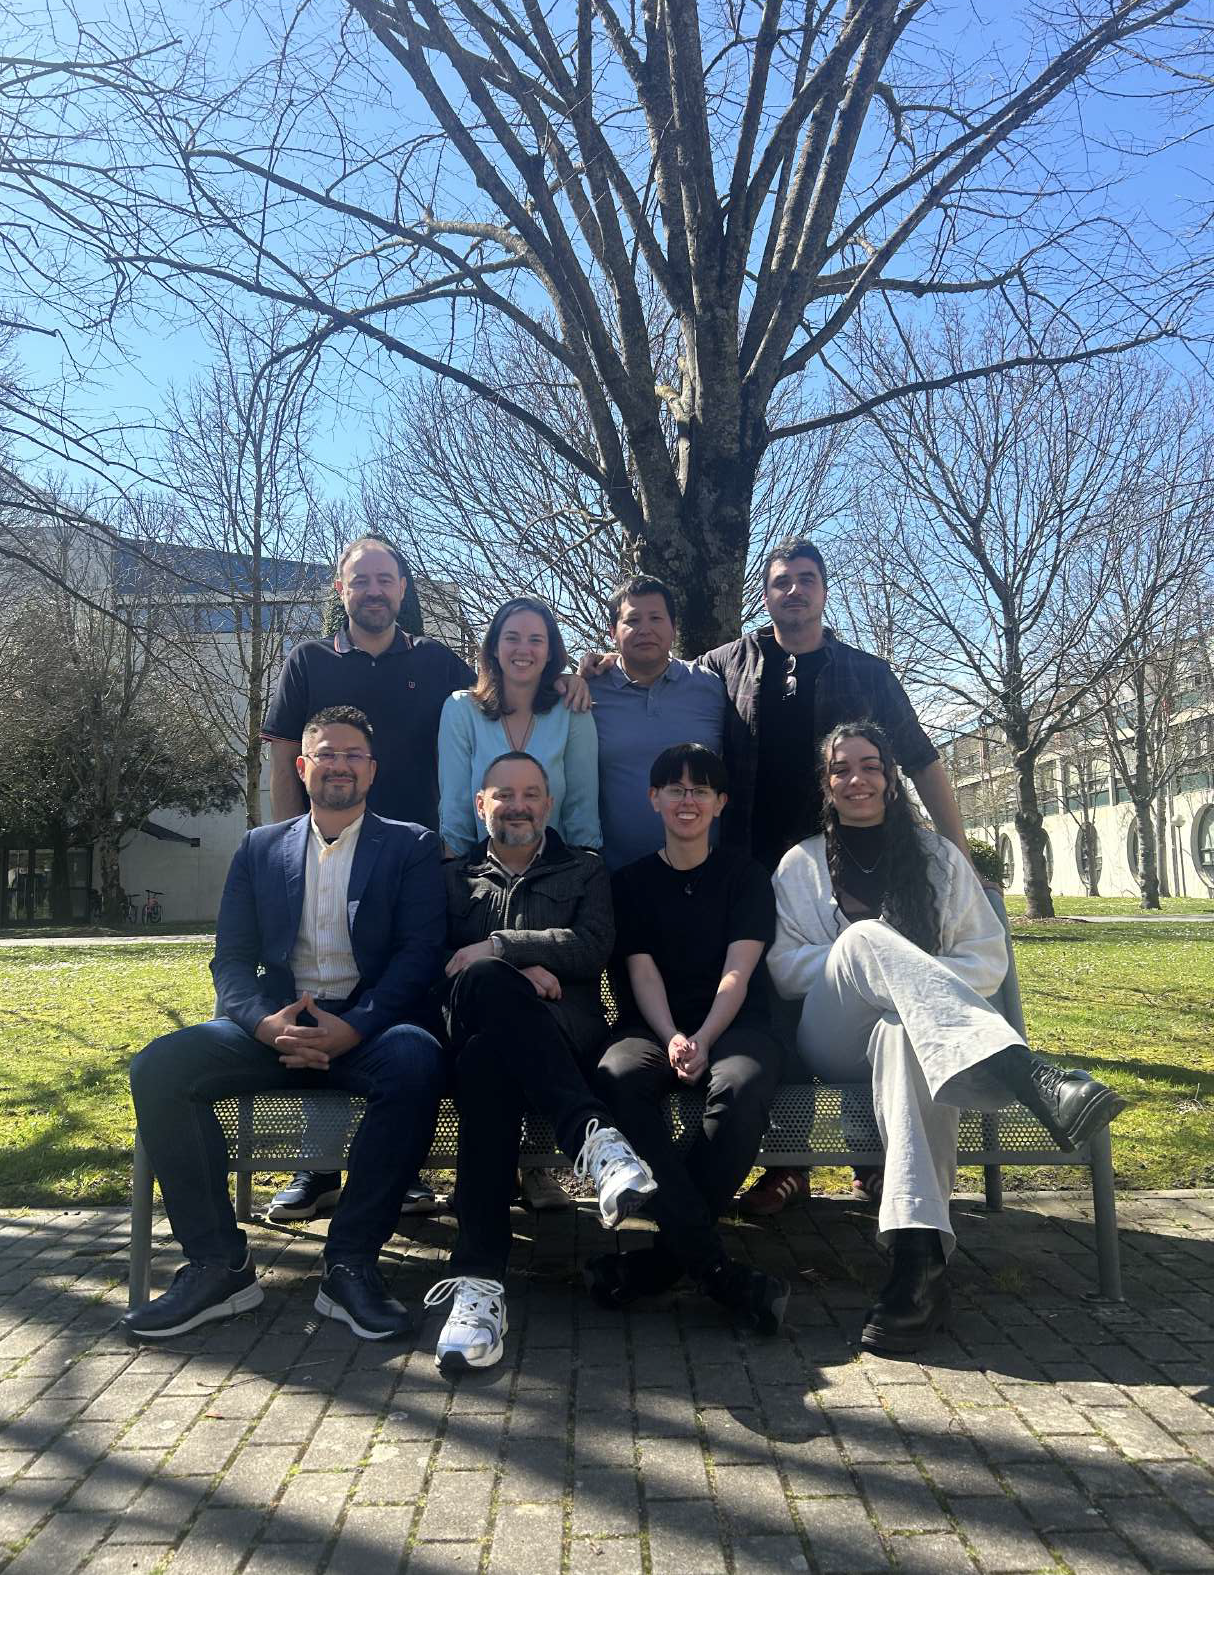
\includegraphics[width=0.85\linewidth]{GR_460.png}
			
		\end{column}
		
	\end{columns}
	
\end{frame}
%------------------------------------------------
\begin{frame}{Contenido} 
	\tableofcontents 
\end{frame}
%------------------------------------------------
\section{Introducción}

\begin{frame}{Importancia de la memoria y el aprendizaje en la infancia}
	
	\centering
	\begin{tikzpicture}[
		block/.style={
			draw,
			rounded corners,
			fill=orange!30,
			text width=0.28\textwidth,
			minimum height=5.5cm,
			align=left,
			font=\scriptsize
		}
		]
		
		% Bloque 1
		\node[block] (b1) {
			\begin{center}
				\textbf{El desarrollo infantil comprende dimensiones:}
			\end{center}
			
			\begin{itemize}
				\item Físicas
				\item Emocionales
				\item Sociales
				\item Cognitivas
			\end{itemize}
		};
		
		% Bloque 2
		\node[block,right=0.4cm of b1] (b2) {
			\begin{center}
				\textbf{La memoria y aprendizaje:}
			\end{center}
			
			\begin{itemize}
				\item Son habilidades cognitivas esenciales
			\end{itemize}
			
			\begin{center}
			\textbf{Alteraciones en estas funciones se observan en:}
		\end{center}
		
		\begin{itemize}
			\item Trastornos del neurodesarrollo (TDAH y TEA).
			\item Trastornos cognitivos y del aprendizaje.
		\end{itemize}
		};
		
		% Bloque 3
		\node[block,right=0.4cm of b2] (b3) {
			\begin{center}
				\textbf{Las dificultades de memoria afectan:}
			\end{center}
			
			\begin{itemize}
				\item Rendimiento académico
				\item Interacción social
				\item Desarrollo del lenguaje
			\end{itemize}
		};
		
		% Flechas
%		\draw[->,thick] (b1) -- (b2);
%		\draw[->,thick] (b2) -- (b3);
		
	\end{tikzpicture}
	
\end{frame}


\begin{frame}{Evaluación neuropsicológica de la memoria}
	
	\centering
	
	\begin{tikzpicture}[
		block/.style={
			draw,
			rounded corners,
			fill=cyan!40,
			text width=0.28\textwidth,
			minimum height=4.5cm,
			align=center,
			font=\small
		}
		]
		
		\node[block] (b1) {
			\textbf{Instrumentos clásicos}
			
			\vspace{0.3cm}
			
			\begin{itemize}
				\item Rey Auditory Verbal Learning Test (RAVLT)\\
				\item California Verbal Learning Test (CVTL)\\
				\item NEUROPSI\\
				\item ENI\\
				\item Rey-Osterrieth
			\end{itemize}
		};
		
		\node[block,right=1cm of b1] (b2) {
			\textbf{Memoria evaluada}
			
			\vspace{0.3cm}
			
			\begin{itemize}
				\item Trabajo\\
				\item Prospectiva\\
				\item Verbal\\
				\item Visual\\
				\item Corto y largo plazo
			\end{itemize}
		};
		
		\node[block,right=1cm of b2] (b3) {
			\textbf{Problema}
			
			\vspace{0.3cm}
			
			\begin{itemize}
			\item Normas escasas\\
			\item Adaptación cultural limitada\\
			\item Costos elevados
		\end{itemize}
		};
		
		\draw[->,thick] (b1) -- (b2);
		\draw[->,thick] (b2) -- (b3);
		
	\end{tikzpicture}
	
\end{frame}

\begin{frame}{Limitaciones de los instrumentos actuales}
	
		\begin{enumerate}
			\item Diseñados originalmente para adultos de EE.UU. y Europa.
			\vspace{7pt}
			\item Escasa adaptación cultural para países latinoamericanos.
			\vspace{7pt}
			\item Normas poblacionales limitadas o inexistentes.
			\vspace{7pt}
			\item Influencia del contexto:
			\begin{itemize}
				\item Nivel educativo de los padres
				\item Condición socioeconómica
				\item Diferencias entre países
			\end{itemize}
			\vspace{7pt}
			\item Alto costo de adquisición.
		\end{enumerate}
	
	\vspace{0.3cm}
	
	\textcolor{red}{\bf Más del 60\% de los neuropsicólogos latinoamericanos reportan falta de normas locales \citep{Arango-Lasprilla04072017}.}
	
\end{frame}


\begin{frame}{Limitaciones de la ENI (Evaluación Neuropsicológica Infantil)}
	
	\begin{itemize}
		\item Desarrollada en México y tiene un amplio uso en Latinoamérica.
		\vspace{7pt}
		\item Evalúa múltiples dominios cognitivos.
		\vspace{7pt}
		\item Aplicación extensa y demandante.
		\vspace{7pt}
		\item Costosa para muchos profesionales.
		\vspace{7pt}
		\item Normativas originalmente mexicanas.
		\vspace{7pt}
		\item Adaptación colombiana basada en:
		\begin{itemize}
			\item Una sola región
			\item Muestra limitada
			\item Modelos estadísticos tradicionales
		\end{itemize}
	\end{itemize}
	
\end{frame}



\begin{frame}{El Test de Aprendizaje y Memoria Verbal (TAMV-I)}
	
	\begin{itemize}
		\item El TAMV-I fue desarrollado para población hispanohablante y cuenta con datos normativos para nueve países latinoamericanos y España \citep{rivera2017}.
		\vspace{7pt}
		\item Edad: 6 a 17 años
		\vspace{7pt}
		\item Licencia abierta.
		\vspace{7pt}
		\item Buenas propiedades psicométricas.
		\vspace{7pt}
		\item Datos normativos para:
		\begin{itemize}
			\item 9 países latinoamericanos
			\item España
		\end{itemize}
	\end{itemize}
	
	\vspace{0.4cm}
	
	\begin{block}{Ventaja}
		Una alternativa accesible para la práctica clínica en Latinoamérica.
	\end{block}
	
\end{frame}


\begin{frame}{Vacío metodológico (GAP)}
	
	\centering
	
	\begin{tikzpicture}[
		block/.style={
			draw,
			rounded corners,
			fill=orange!20,
			text width=0.5\textwidth,
			align=center,
			font=\small,
			minimum height=1.5cm
		},
		smallblock/.style={
			draw,
			rounded corners,
			fill=blue!15,
			text width=0.22\textwidth,
			align=center,
			font=\scriptsize,
			minimum height=2.8cm
		}
		]
		
		% Problema principal
		\node[block] (main) {
			\textbf{Problema}
			
			Las normas del TAMV-I suelen estimarse mediante modelos univariados
			que asumen independencia entre las puntuaciones.
		};
		
		% Razón 1
	\node[smallblock, below left=0.8cm and 0.2cm of main] (b1) {
			\textbf{1. Dependencia entre puntuaciones}
			
			Las puntuaciones del TAMV-I están correlacionadas.
			
			\vspace{0.2cm}
			
			Los análisis univariados no capturan esta estructura.
		};
		
		% Razón 2
		\node[smallblock, below=0.8cm of main] (b2) {
			\textbf{2. Error estadístico}
			
			Se requieren múltiples modelos independientes.
			
			\vspace{0.2cm}
			
			$\uparrow$ Error Tipo I
			
			$\downarrow$ Potencia estadística
		};
		
		% Razón 3
		\node[smallblock, below right=0.8cm and 0.2cm of main] (b3) {
			\textbf{3. Falta de parsimonia}
			
			Un modelo para cada puntuación.
			
			\vspace{0.2cm}
			
			Mayor complejidad analítica de la necesaria.
		};
		
		\draw[->,thick] (main) -- (b1);
		\draw[->,thick] (main) -- (b2);
		\draw[->,thick] (main) -- (b3);
		
	\end{tikzpicture}
	
\end{frame}

\begin{frame}{Propuesta metodológica}
	\vspace{-1cm}
	\begin{columns}[T]
		
		%---------------------------
		% Columna izquierda
		%---------------------------
		\begin{column}{0.45\textwidth}
			
	
				\begin{center}
						\textcolor{blue}{\bf Enfoque tradicional}\\
					\textbf{Teoría Clásica de los Tests (TCT)}\\
					\vspace{0.2cm}
					\Large $\Downarrow$\\
					\vspace{0.2cm}
					\textcolor{red}{\small Limitaciones}
				\end{center}
				
				\begin{itemize}
					\item Error de medida constante
					\item Análisis univariados
					\item Dependencia de la muestra
					\item Menor precisión psicométrica
				\end{itemize}
			
		\end{column}
		
		%---------------------------
		% Columna derecha
		%---------------------------
		\begin{column}{0.55\textwidth}
		
	
			\begin{center}
					\textcolor{blue}{\bf Propuesta del estudio}\\
				\textbf{IRT}\\
				\vspace{0.1cm}
				\Large +\\
				\vspace{0.1cm}
				\textbf{\small Modelos Lineales Mixtos (LMM)}\\
				\textcolor{red}{\small Ventajas}
			\end{center}
			
			
			
			\begin{itemize}
					\item Modela dificultad y discriminación.
					\item Captura correlación entre ensayos.
					\item Ajusta covariables demográficas.
					\item Produce normas más precisas.
			\end{itemize}
			
		\end{column}
		
	\end{columns}
	
\end{frame}


\begin{frame}{Propósito}
	
	\begin{block}{Objetivo general}
		
		Desarrollar datos normativos para el
		Test de Aprendizaje y Memoria Verbal
		(TAMV-I) combinando:
		
		\begin{center}
			
			\Large
			IRT + Modelos Mixtos
			
		\end{center}
		
		con el fin de generar estimaciones
		normativas más robustas y precisas para
		niños y adolescentes hispanohablantes.
		
	\end{block}
	
\end{frame}

%------------------------------------------------
\section{Métodos}
%------------------------------------------------
\subsection{Participantes}

\begin{frame}{Participantes I}
	
	\centering
	
	\begin{tikzpicture}[
		block/.style={
			draw,
			rounded corners,
			fill=red!15,
			text width=0.3\textwidth,
			minimum height=5cm,
			align=center,
			font=\small,
		}
		]
		
		\node[block] (b1) {
			\textbf{Muestra}
			\vspace{0.2cm}
			\begin{itemize}
				\item 1.748 participantes de:
				\begin{itemize}
					\item[$\bullet$] España (399)
					\item[$\bullet$] Honduras (288)
					\item[$\bullet$] Colombia (457)
					\item[$\bullet$] Ecuador (604)
				\end{itemize}
				\item 1.640 casos completos (muestra final)
			\end{itemize}
		};
		
		\node[block,right=0.5cm of b1] (b2) {
			\textbf{Características sociodemográficas}
			\vspace{0.2cm}
			\begin{itemize} 
				\item 52,56\% mujeres 
				\item Edad media: 11,19 años (DE = 3,36) 
				\item Escolaridad parental media: 13,32 años (DE = 3,87) 
			\end{itemize}
		};
		
		\node[block,right=0.5cm of b2] (b3) {
			\textbf{Calidad de la muestra}
			\vspace{0.2cm}
			\begin{itemize} 
				\item Distribución balanceada por sexo y edad. 
				\item Escolaridad parental monitoreada en cada país. 
				\item Errores estándar dentro de rangos aceptables (Nivel de confianza: 95\%)
			 \end{itemize}
		};
	\end{tikzpicture}
\end{frame}


\begin{frame}{Participantes II}
	\vspace{-0.5cm}
	\small
	\begin{columns}[T]
		
		\begin{column}{0.48\textwidth}
			
			\begin{block}{Criterios de inclusión}
				\begin{itemize}
					\item Edad entre 6 y 17 años.
					\item Nacidos en España, Honduras, Colombia o Ecuador.
					\item CI $\geq$ 80 (TONI-2).
					\item Puntaje $<$ 19 en el Children's Depression Inventory.
				\end{itemize}
			\end{block}
			
		\end{column}
		
		\begin{column}{0.48\textwidth}
			
			\begin{alertblock}{Criterios de exclusión}
				\begin{itemize}
					\item Trastornos neurológicos con impacto cognitivo.
					\item Trastornos psiquiátricos.
					\item Discapacidad intelectual o trastornos del neurodesarrollo.
					\item Enfermedades sistémicas no controladas.
					\item Déficits sensoriales severos.
					\item Complicaciones pre-, peri- o postnatales.
					\item Consumo de alcohol o sustancias psicoactivas.
				\end{itemize}
			\end{alertblock}
		\end{column}
	\end{columns}
\end{frame}

%\begin{frame}{Participantes III}
%	\vspace{-0.4cm}
%	\begin{figure}
%		\centering
%		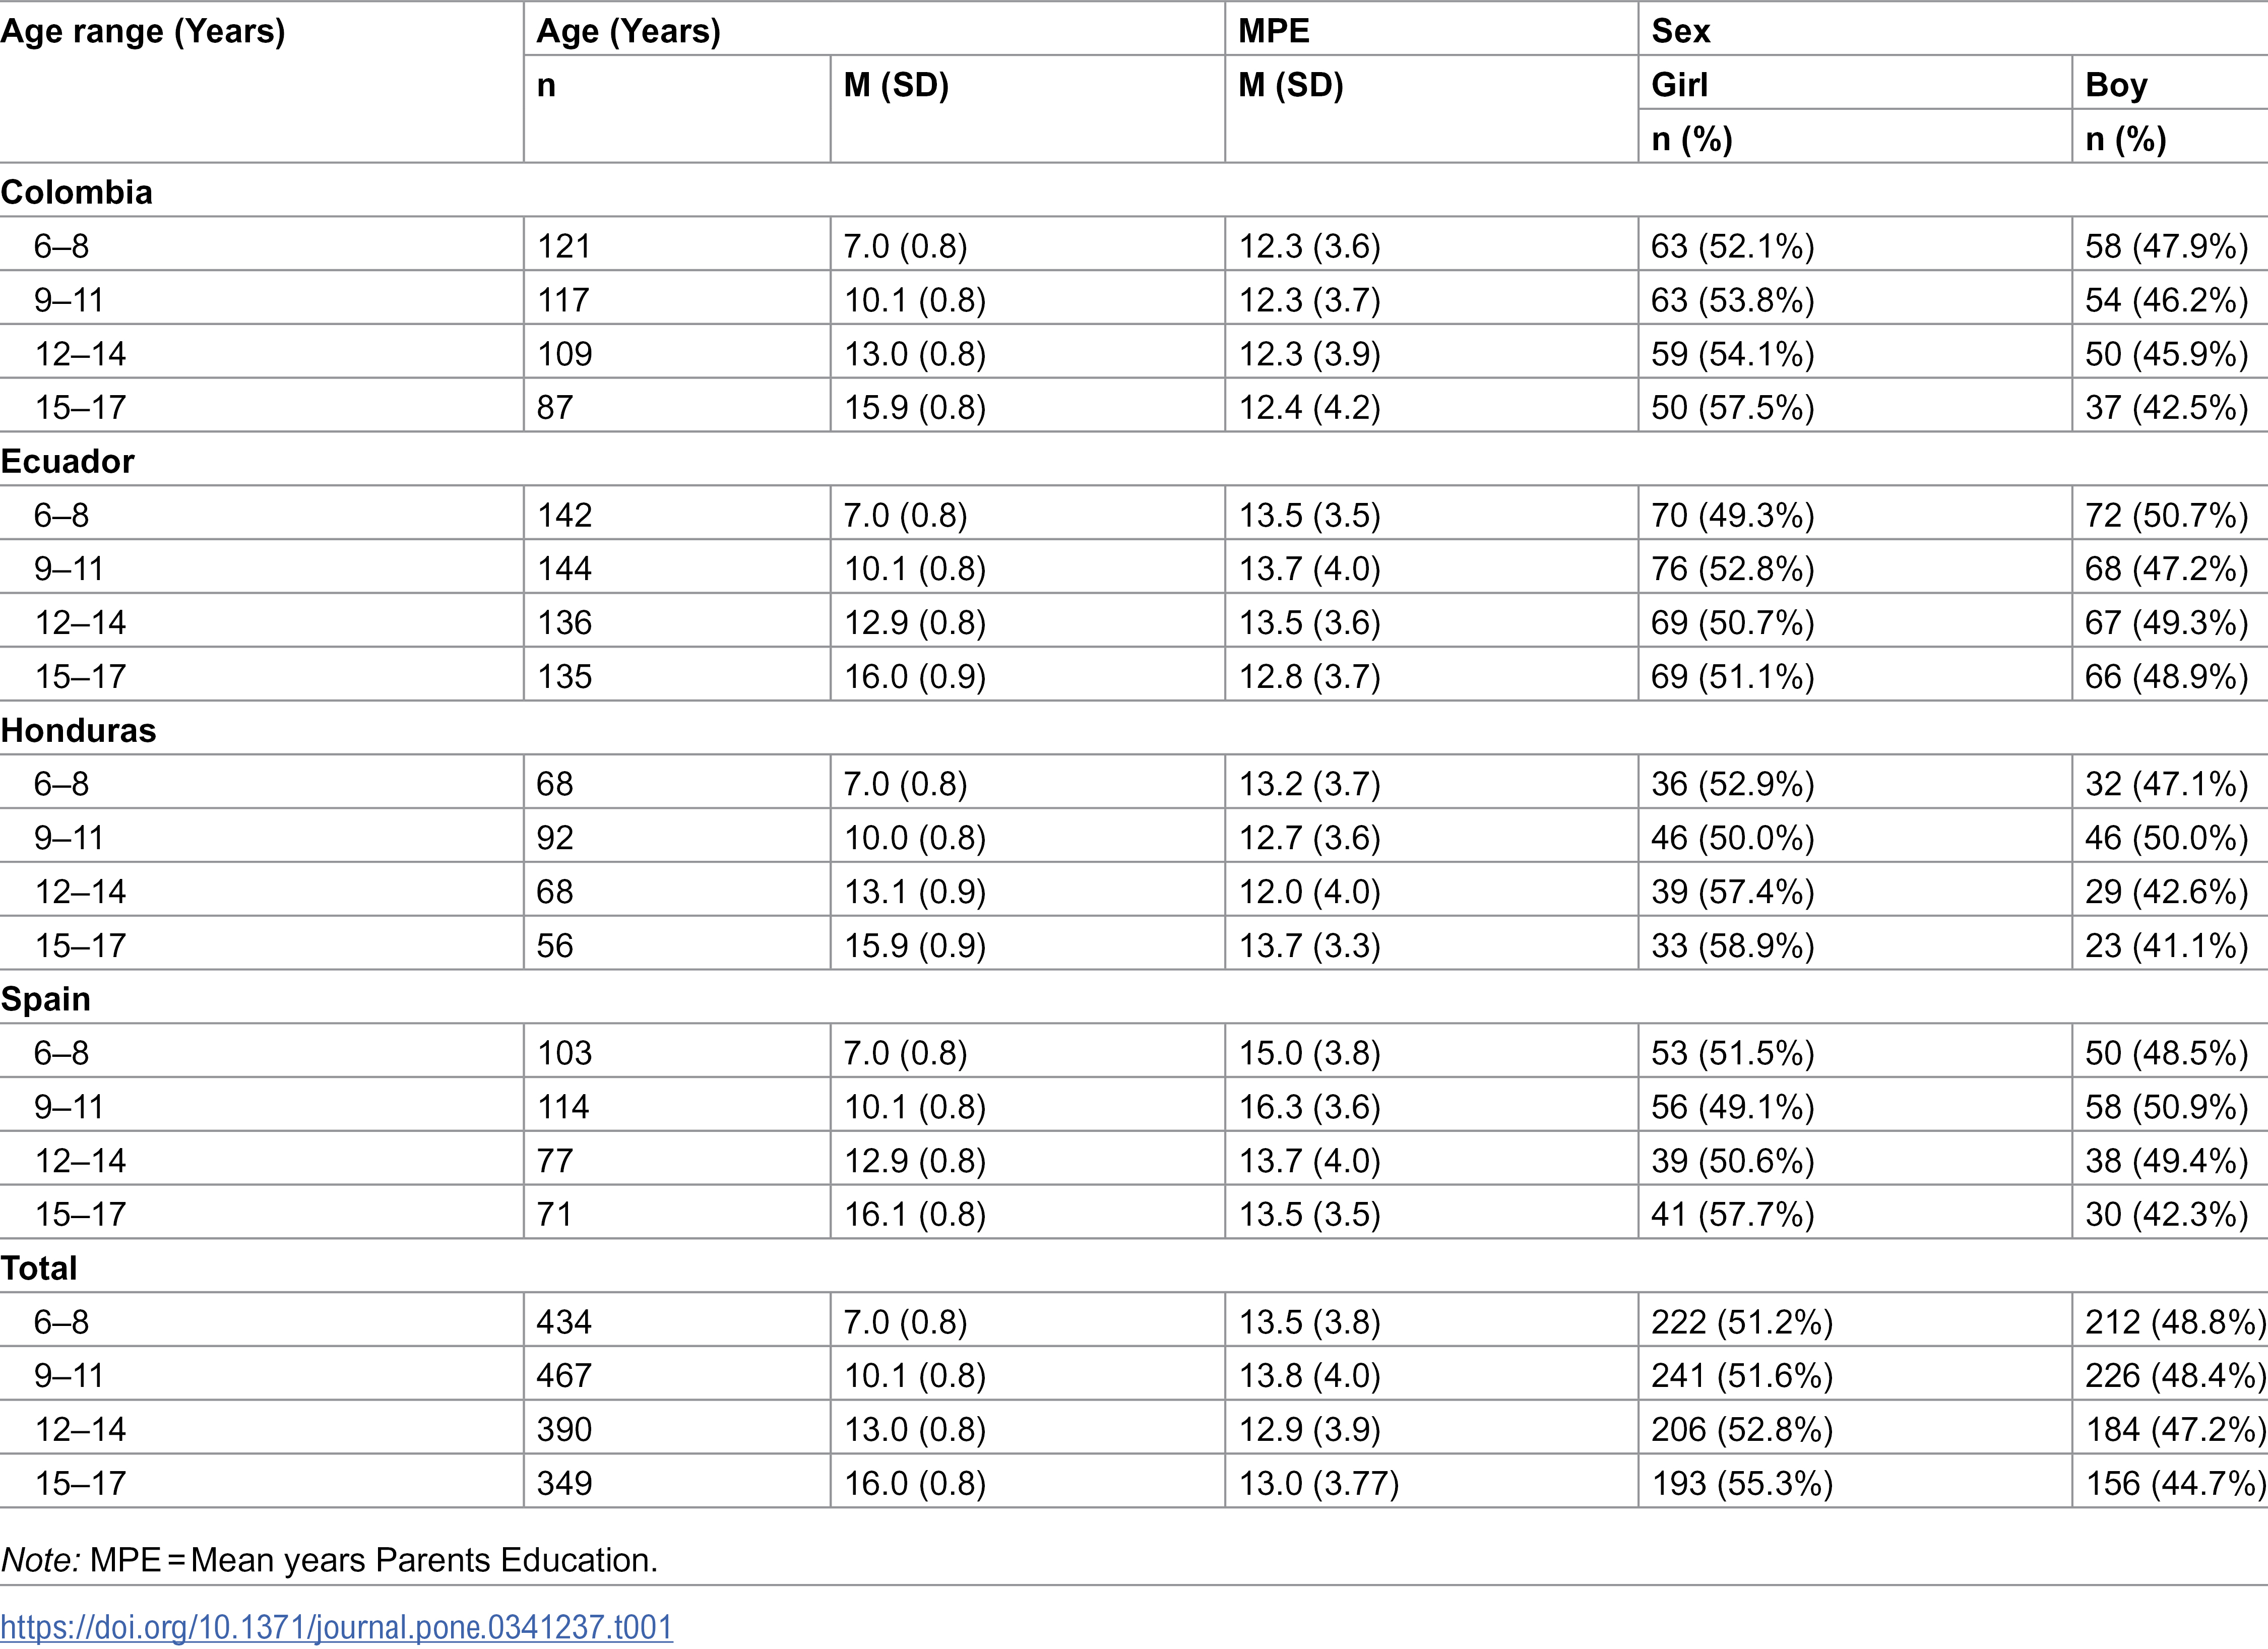
\includegraphics[width=0.65\linewidth]{journal.pone.0341237.t001}
%		\caption{}
%		\label{fig:journal}
%	\end{figure}
%	
%\end{frame}

\subsection{Instrumento}

\begin{frame}{Test de Aprendizaje y Memoria Verbal (TAMV-I)}
	\vspace{-0.4cm}
	\centering
	
	\begin{tikzpicture}[
		block/.style={
			draw,
			rounded corners,
			fill=green!15,
			text width=0.28\textwidth,
			minimum height=5cm,
			align=center,
			font=\small
		}
		]
		
		% Bloque 1
		\node[block] (b1) {
			\textbf{Recuerdo Libre}
			
			\vspace{0.2cm}
			
			4 ensayos
			
			\vspace{0.2cm}
			
			Lista de 12 palabras
			
			\begin{itemize}
				\item Ropa
				\item Muebles
				\item Partes del cuerpo
			\end{itemize}
			
			Máximo: 48 puntos
		};
		
		% Bloque 2
		\node[block,right=0.6cm of b1] (b2) {
			\textbf{Recuerdo Diferido}
			
			\vspace{0.2cm}
			
			30 minutos después
			
			\vspace{0.2cm}
			
			Evocación de las palabras recordadas
			
			\vspace{0.5cm}
			
			Máximo: 12 puntos
		};
		
		% Bloque 3
		\node[block,right=0.6cm of b2] (b3) {
			\textbf{Reconocimiento}
			
			\vspace{0.2cm}
			
			48 palabras
			
			\begin{itemize}
				\item 12 originales
				\item 12 semánticamente relacionadas
				\item 12 fonológicamente relacionadas
				\item 12 no relacionadas
			\end{itemize}
			
			Máximo: 12 puntos
		};
		
		\draw[->,thick] (b1) -- (b2);
		\draw[->,thick] (b2) -- (b3);
		
	\end{tikzpicture}
	
	\begin{alertblock}{Puntuación}
		Se asigna 1 punto por cada palabra correctamente recordada o reconocida.
	\end{alertblock}
\end{frame}

\subsection{Procedimiento}

\begin{frame}{Procedimiento y consideraciones éticas}
	\scriptsize
	\begin{block}{Diseño del estudio}
		\begin{itemize}
			\item Parte de un proyecto internacional para generar normas neuropsicológicas en Latinoamérica y España.
			\item Aprobado por comités de ética de España, Colombia, Ecuador y Honduras.
		\end{itemize}
	\end{block}
	
	\begin{block}{Recolección de datos}
		\begin{itemize}
			\item Periodo: marzo de 2016 a junio de 2017.
			\item Convenios con instituciones educativas de cada país.
			\item Participación voluntaria de estudiantes y sus familias.
		\end{itemize}
	\end{block}
	
	\begin{block}{Evaluación}
		\begin{itemize}
			\item Consentimiento informado y asentimiento según la edad.
			\item Aplicación individual de la batería neuropsicológica.
			\item Duración aproximada: 120 minutos.
			\item Sin incentivos económicos.
		\end{itemize}
	\end{block}
	
\end{frame}


\subsection{Análisis estadístico}

\begin{frame}{Parámetros de los ítems y estimación de la habilidad ($\theta$) I}
	\begin{itemize}
		\item Para determinar los parámetros de los ítems (dificultad y discriminación) se usó Teoría de Respuesta al Ítem (IRT, siglas en inglés).
		\vspace{10pt}
		\item Debido a la naturaleza dicotómica de los datos, se ajustaron los modelos Rasch y 2PL.
		\vspace{10pt}
		\item Razón de verosimilitud (Likelihood Ratio Test, LRT) y Criterio de Información Bayesiano (BIC) para comparar modelos e identificar el modelo con el mejor ajuste.
	\end{itemize}
\end{frame}

\begin{frame}{Parámetros de los ítems y estimación de la habilidad ($\theta$) II}
	\begin{itemize}
		\item El modelo de Rasch asume una discriminación constante para todos los ítems. El modelo se define de la siguiente manera:
		\[ \log\left(\frac{\pi_i}{1-\pi_i}\right)=\beta_i+\beta z .\]
		Donde:
		\begin{itemize} 
			\item $\pi_i$: probabilidad de respuesta correcta del ítem $i$ dado un nivel de habilidad $z$
			\item $\beta_i$: dificultad (facilidad) del ítem. 
			\item $\beta$: discriminación de los ítems. 
			\item $z$: habilidad latente del participante. 
		\end{itemize}
		\vspace{10pt}
		\item \textcolor{red}{\bf Pero... ¿Qué pasa si la discriminación varía entre ítems?}
	\end{itemize}
\end{frame}

\begin{frame}{Parámetros de los ítems y estimación de la habilidad ($\theta$) III}
	\begin{itemize}
		\item El modelo de dos parámetros (2 PL)  extiende el modelo de Rasch al permitir que los ítems difieran en la nitidez con la que separan a evaluados de distintos niveles de habilidad, se escribe:
		\[ \log\left(\frac{\pi_i}{1-\pi_i}\right)=\beta_{1i}(z-\beta_{0i})\]
		Donde:
		\begin{itemize} 
			\item $\pi_i$: probabilidad de respuesta correcta del ítem $i$
			\item $\beta_{1i}$: parámetro de discriminación.
			\item $\beta_{0i}$: dificultad (facilidad) del ítem. 
			\item $z$: habilidad latente del participante. 
		\end{itemize}
	\end{itemize}
\end{frame}

\begin{frame}{Parámetros de los ítems y estimación de la habilidad ($\theta$) IV}
	\begin{itemize}
		\item Una vez seleccionado el modelo con mejor ajuste, los parámetros de los ítems se utilizaron para estimar la puntuación de habilidad de cada participante $\theta$\\
		\vspace{10pt}
		\item La estimación considera:
		\begin{itemize}
			 \item Dificultad del ítem 
			 \item Discriminación del ítem 
		\end{itemize}
		\vspace{10pt}
		\item Proporciona una medida más precisa que los puntajes brutos. 
		\vspace{10pt}
		\item Se calculó para: 
		\begin{itemize} 
			\item Ensayos 1--4 
			\item Recuerdo diferido 
			\item Reconocimiento 
		\end{itemize}
	\end{itemize}
\end{frame}

\begin{frame}{Efectos demográficos I}
	\begin{itemize}
		\item Para examinar la influencia de los factores demográficos sobre las puntuaciones de habilidad ($\theta$), se aplicaron Modelos Lineales Mixtos (LMM, por sus siglas en inglés).
		\vspace{10pt}
		\item LMM's permiten incluir tanto efectos fijos (ensayo, edad, $edad^2$, sexo, escolaridad parental promedio [MPE], país e interacciones de segundo nivel entre estas variables) como efectos aleatorios, con el fin de capturar la variabilidad intraindividual presente en las mediciones repetidas.
		\vspace{10pt}
		\item Los LMM permiten modelar conjuntamente múltiples resultados correlacionados, lo que significa que todas las puntuaciones de los ensayos se analizan dentro de un mismo marco estadístico.
	\end{itemize}
\end{frame}


\begin{frame}{Efectos demográficos II}
	\begin{itemize}
		\item El modelo se puede escribir:
			\[\theta_{ij} = \beta_0+b_{0i} +\beta_1X_{1ij} +\cdots+ \beta_kX_{kij} +\varepsilon_{ij}\]
				\begin{itemize}
				\item[$\bullet$] $\theta_{ij}$: habilidad del individuo $i$ en el ensayo $j$
				\item[$\bullet$] $\beta$: efectos fijos
				\item[$\bullet$] $b_{0i}$: efectos aleatorios
				\item[$\bullet$] $\varepsilon_{ij}$: error residual
			\end{itemize}
		\vspace{10pt}
		\item La estimación se realiza usando la máxima verosimilitud restringida (REML).
			\vspace{10pt}
			\item El costo computacional proviene de REML debido a la inversión/factorización de matrices dispersas (\textit{sparse}), con una complejidad de $\mathcal{O}(n^{1.5})$ a $\mathcal{O}(n^3)$.
			\vspace{10pt}
			\item El mejor modelo se determina secuencialmente usando el BIC.
	\end{itemize}

\end{frame}

\begin{frame}{Procedimiento de datos normativos}
	\vspace{-0.5cm}
	\begin{figure}
		\centering
		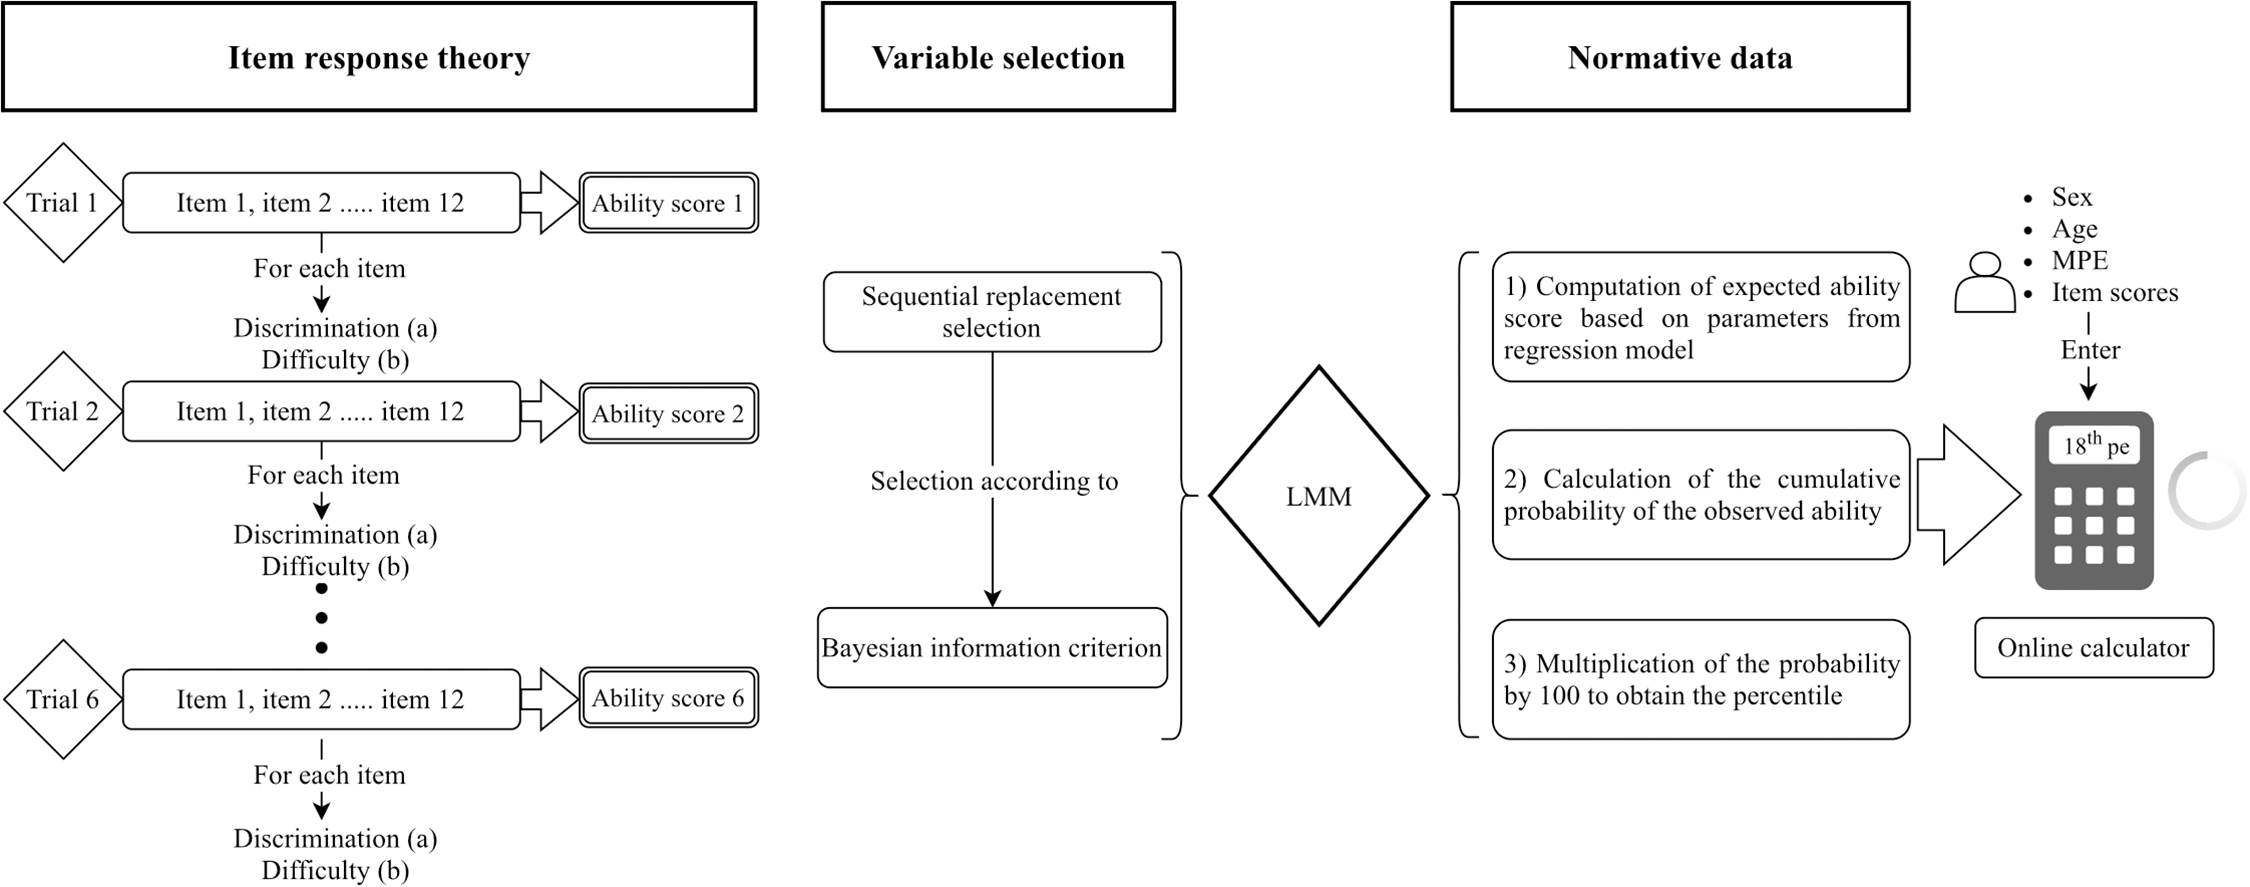
\includegraphics[width=\linewidth]{journal.pone.0341237.g001}
		\label{fig:journalj}
	\end{figure}	
	
\end{frame}

\begin{frame}{Disponibilidad de los datos}
	\centering
	\textbf{Datos disponibles en Zenodo}
	\begin{figure}
		\centering
		
\includegraphics[width=0.4\linewidth]{datos}
		\label{fig:datos}
	\end{figure}
	
\end{frame}

\section{Resultados}

\subsection{Parámetros de los ítems y puntuaciones de las habilidades}

\begin{frame}{Parámetros de los ítems y puntuaciones de las habilidades I}
	\vspace{-1cm}
	\begin{figure}
		\centering
		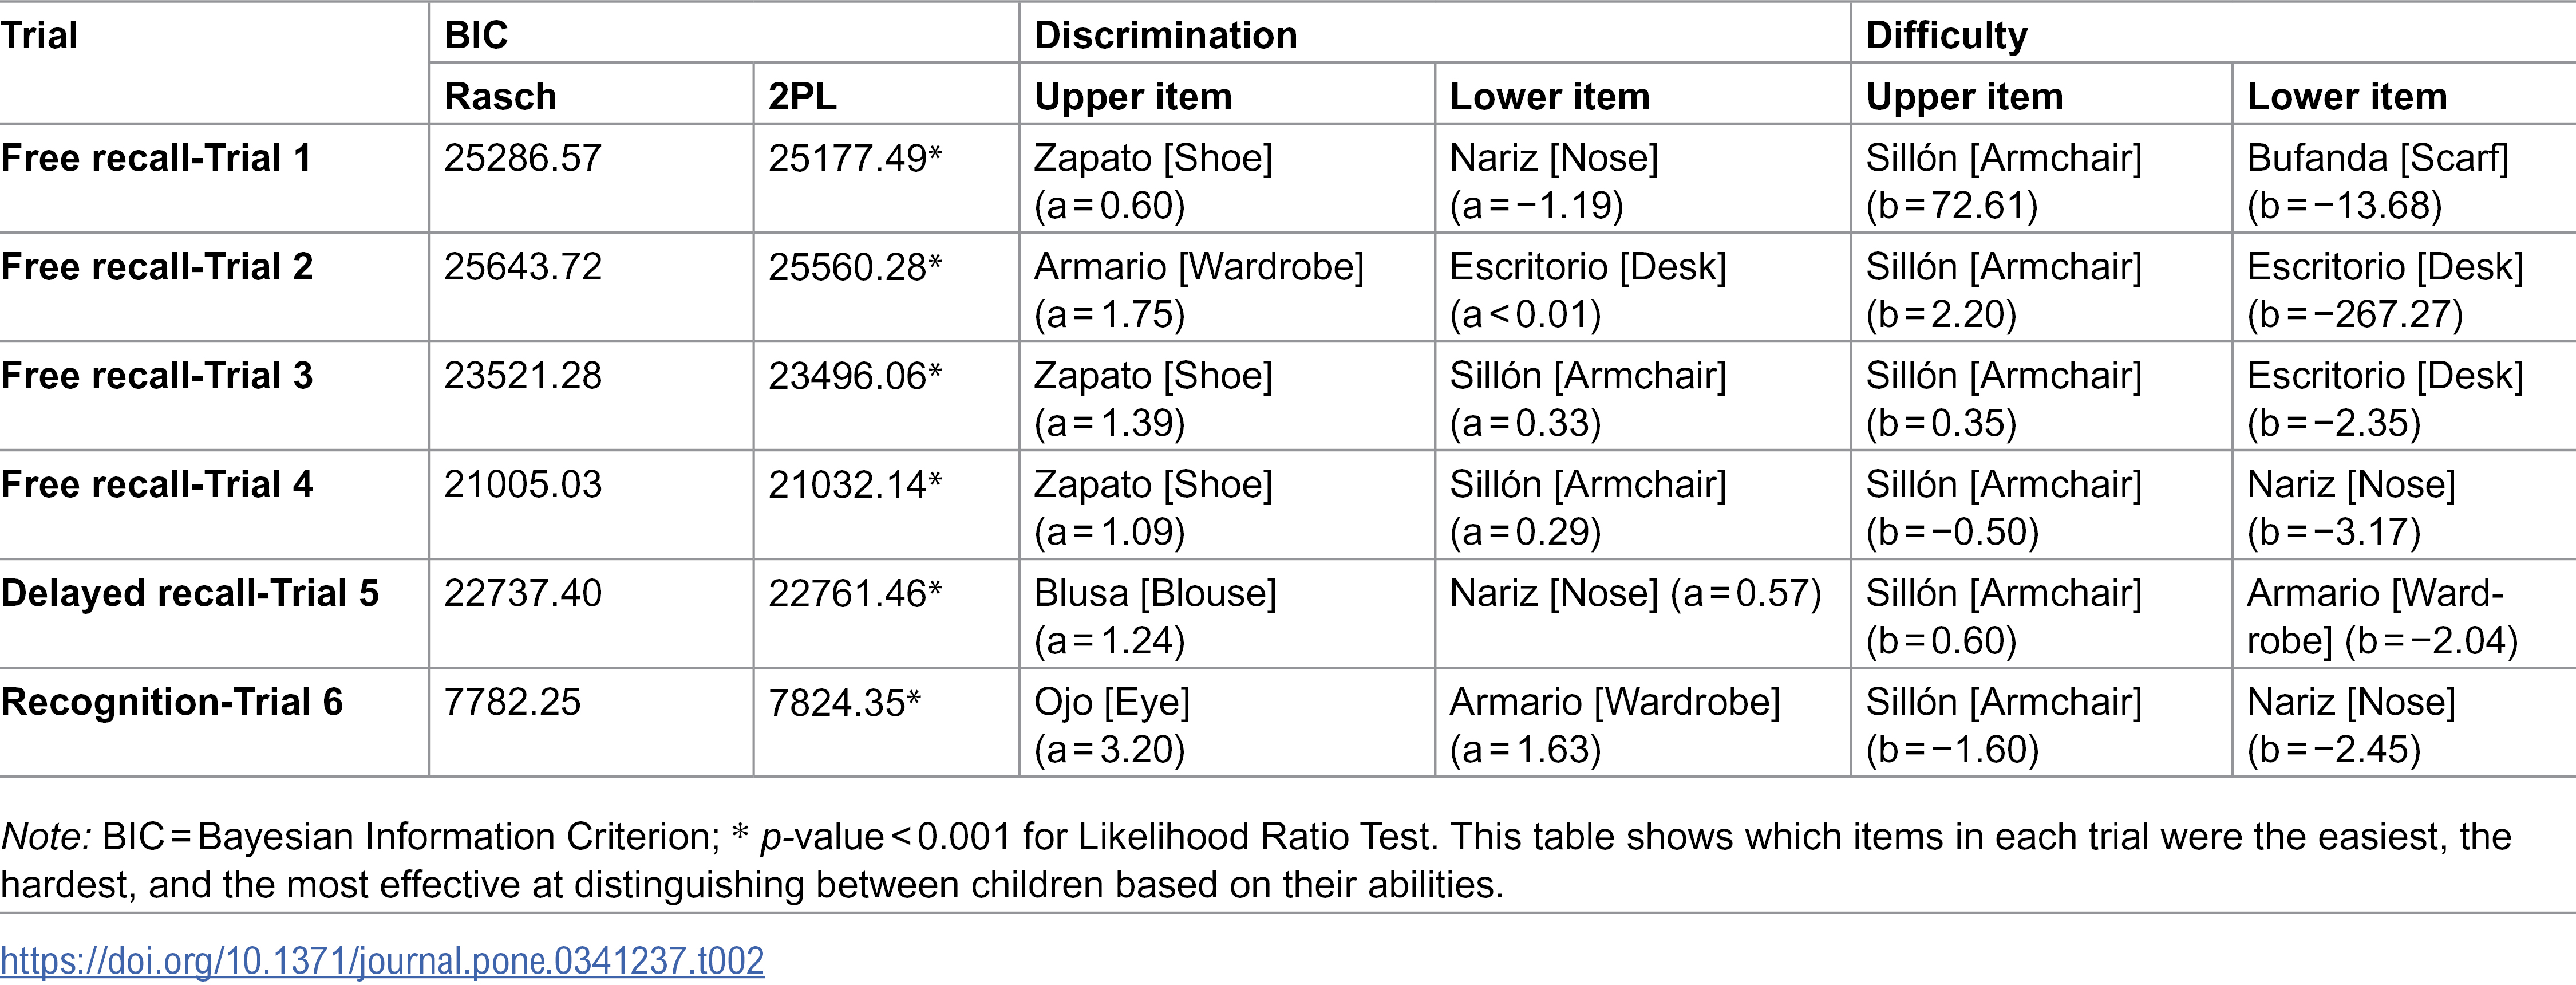
\includegraphics[width=1.05\linewidth]{journal.pone.0341237.t002}
		\label{fig:journalh}
	\end{figure}
\end{frame}

\begin{frame}{Parámetros de los ítems y puntuaciones de las habilidades II}
\begin{figure}
	\centering
	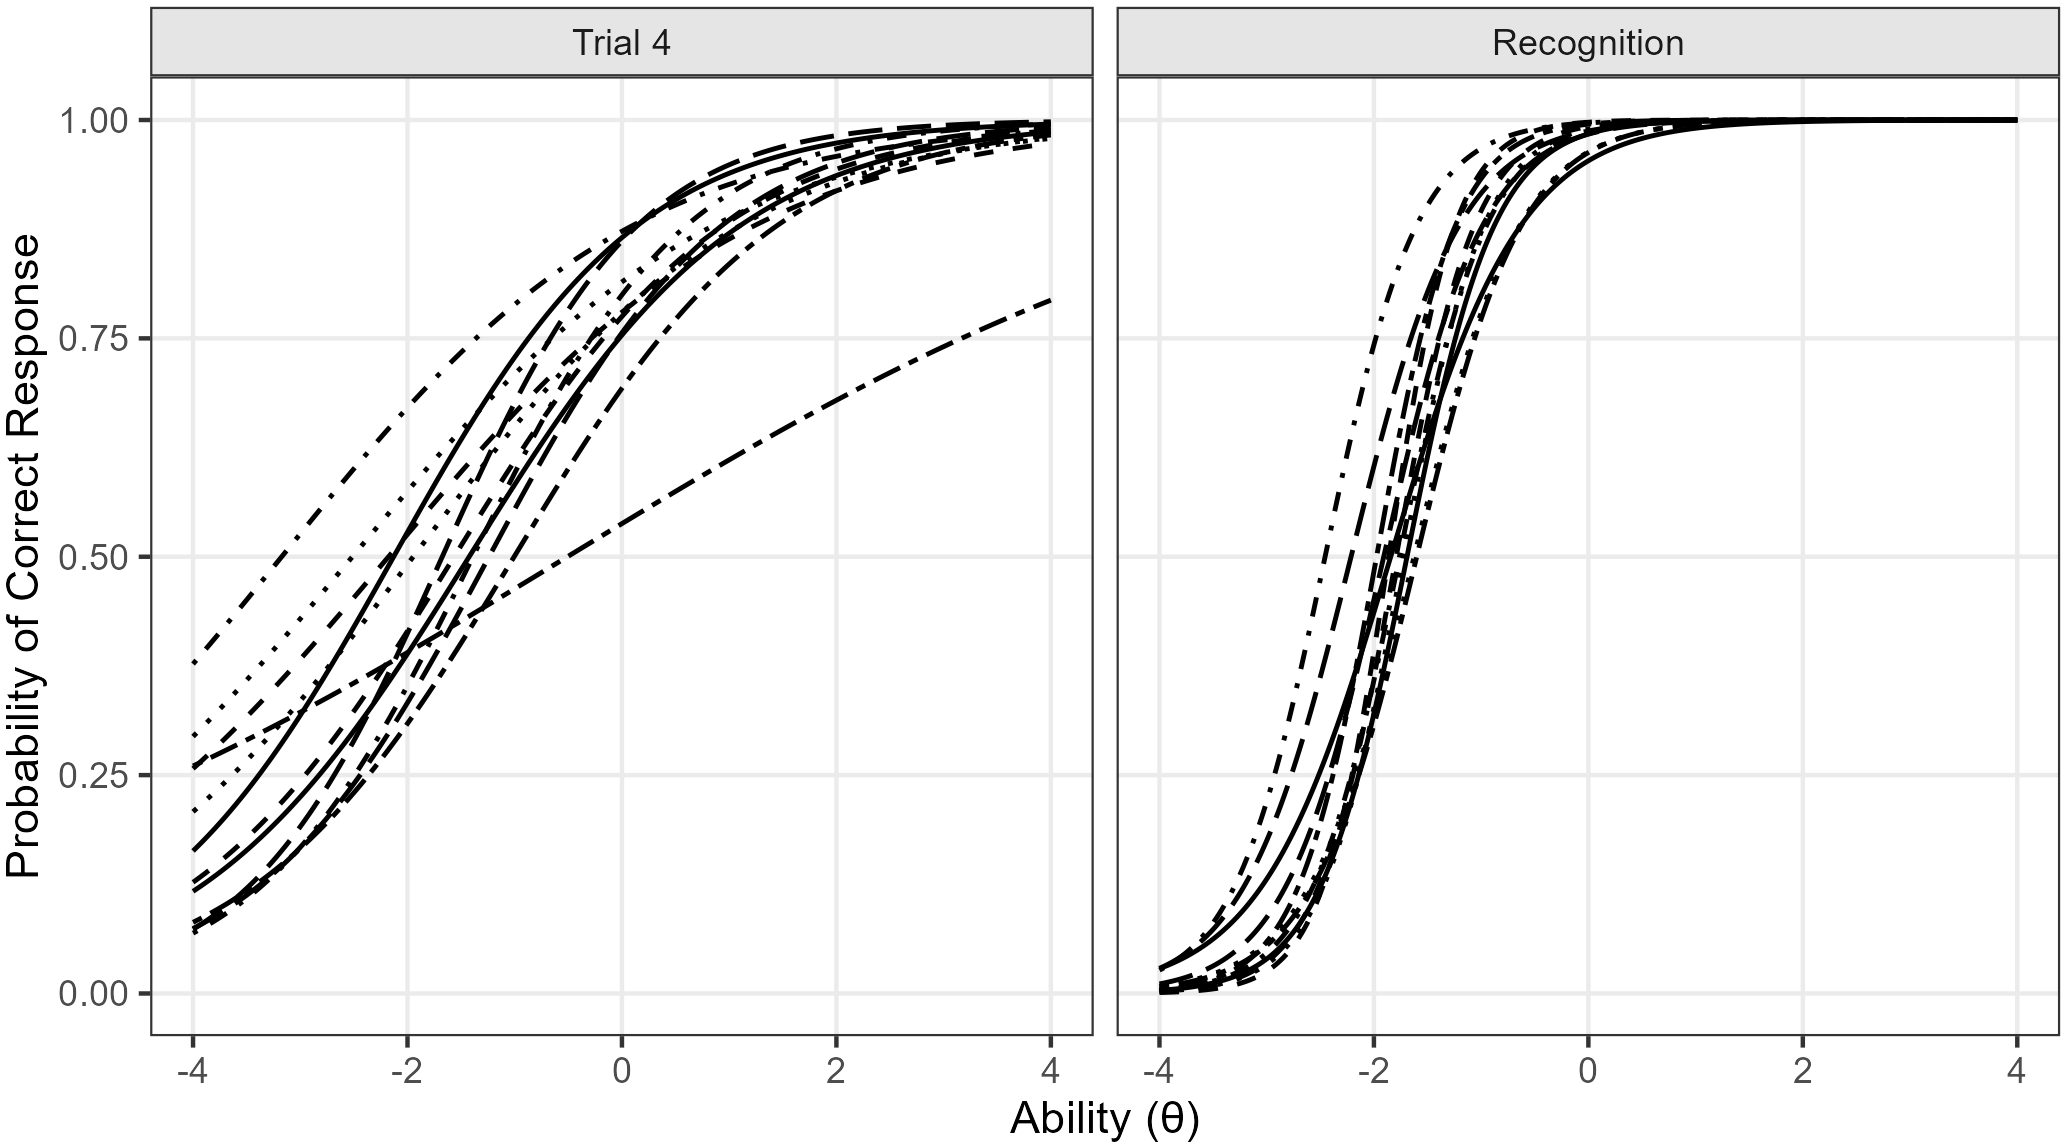
\includegraphics[width=0.7\linewidth]{journal.pone.0341237.g002}
	\label{fig:journall}
\end{figure}
\end{frame}

\subsection{Efecto de las variables demográficas en la habilidad}

\begin{frame}{Efecto de las variables demográficas en la habilidad I}
	\vspace{-0.5cm}
	\begin{figure}
			\centering
			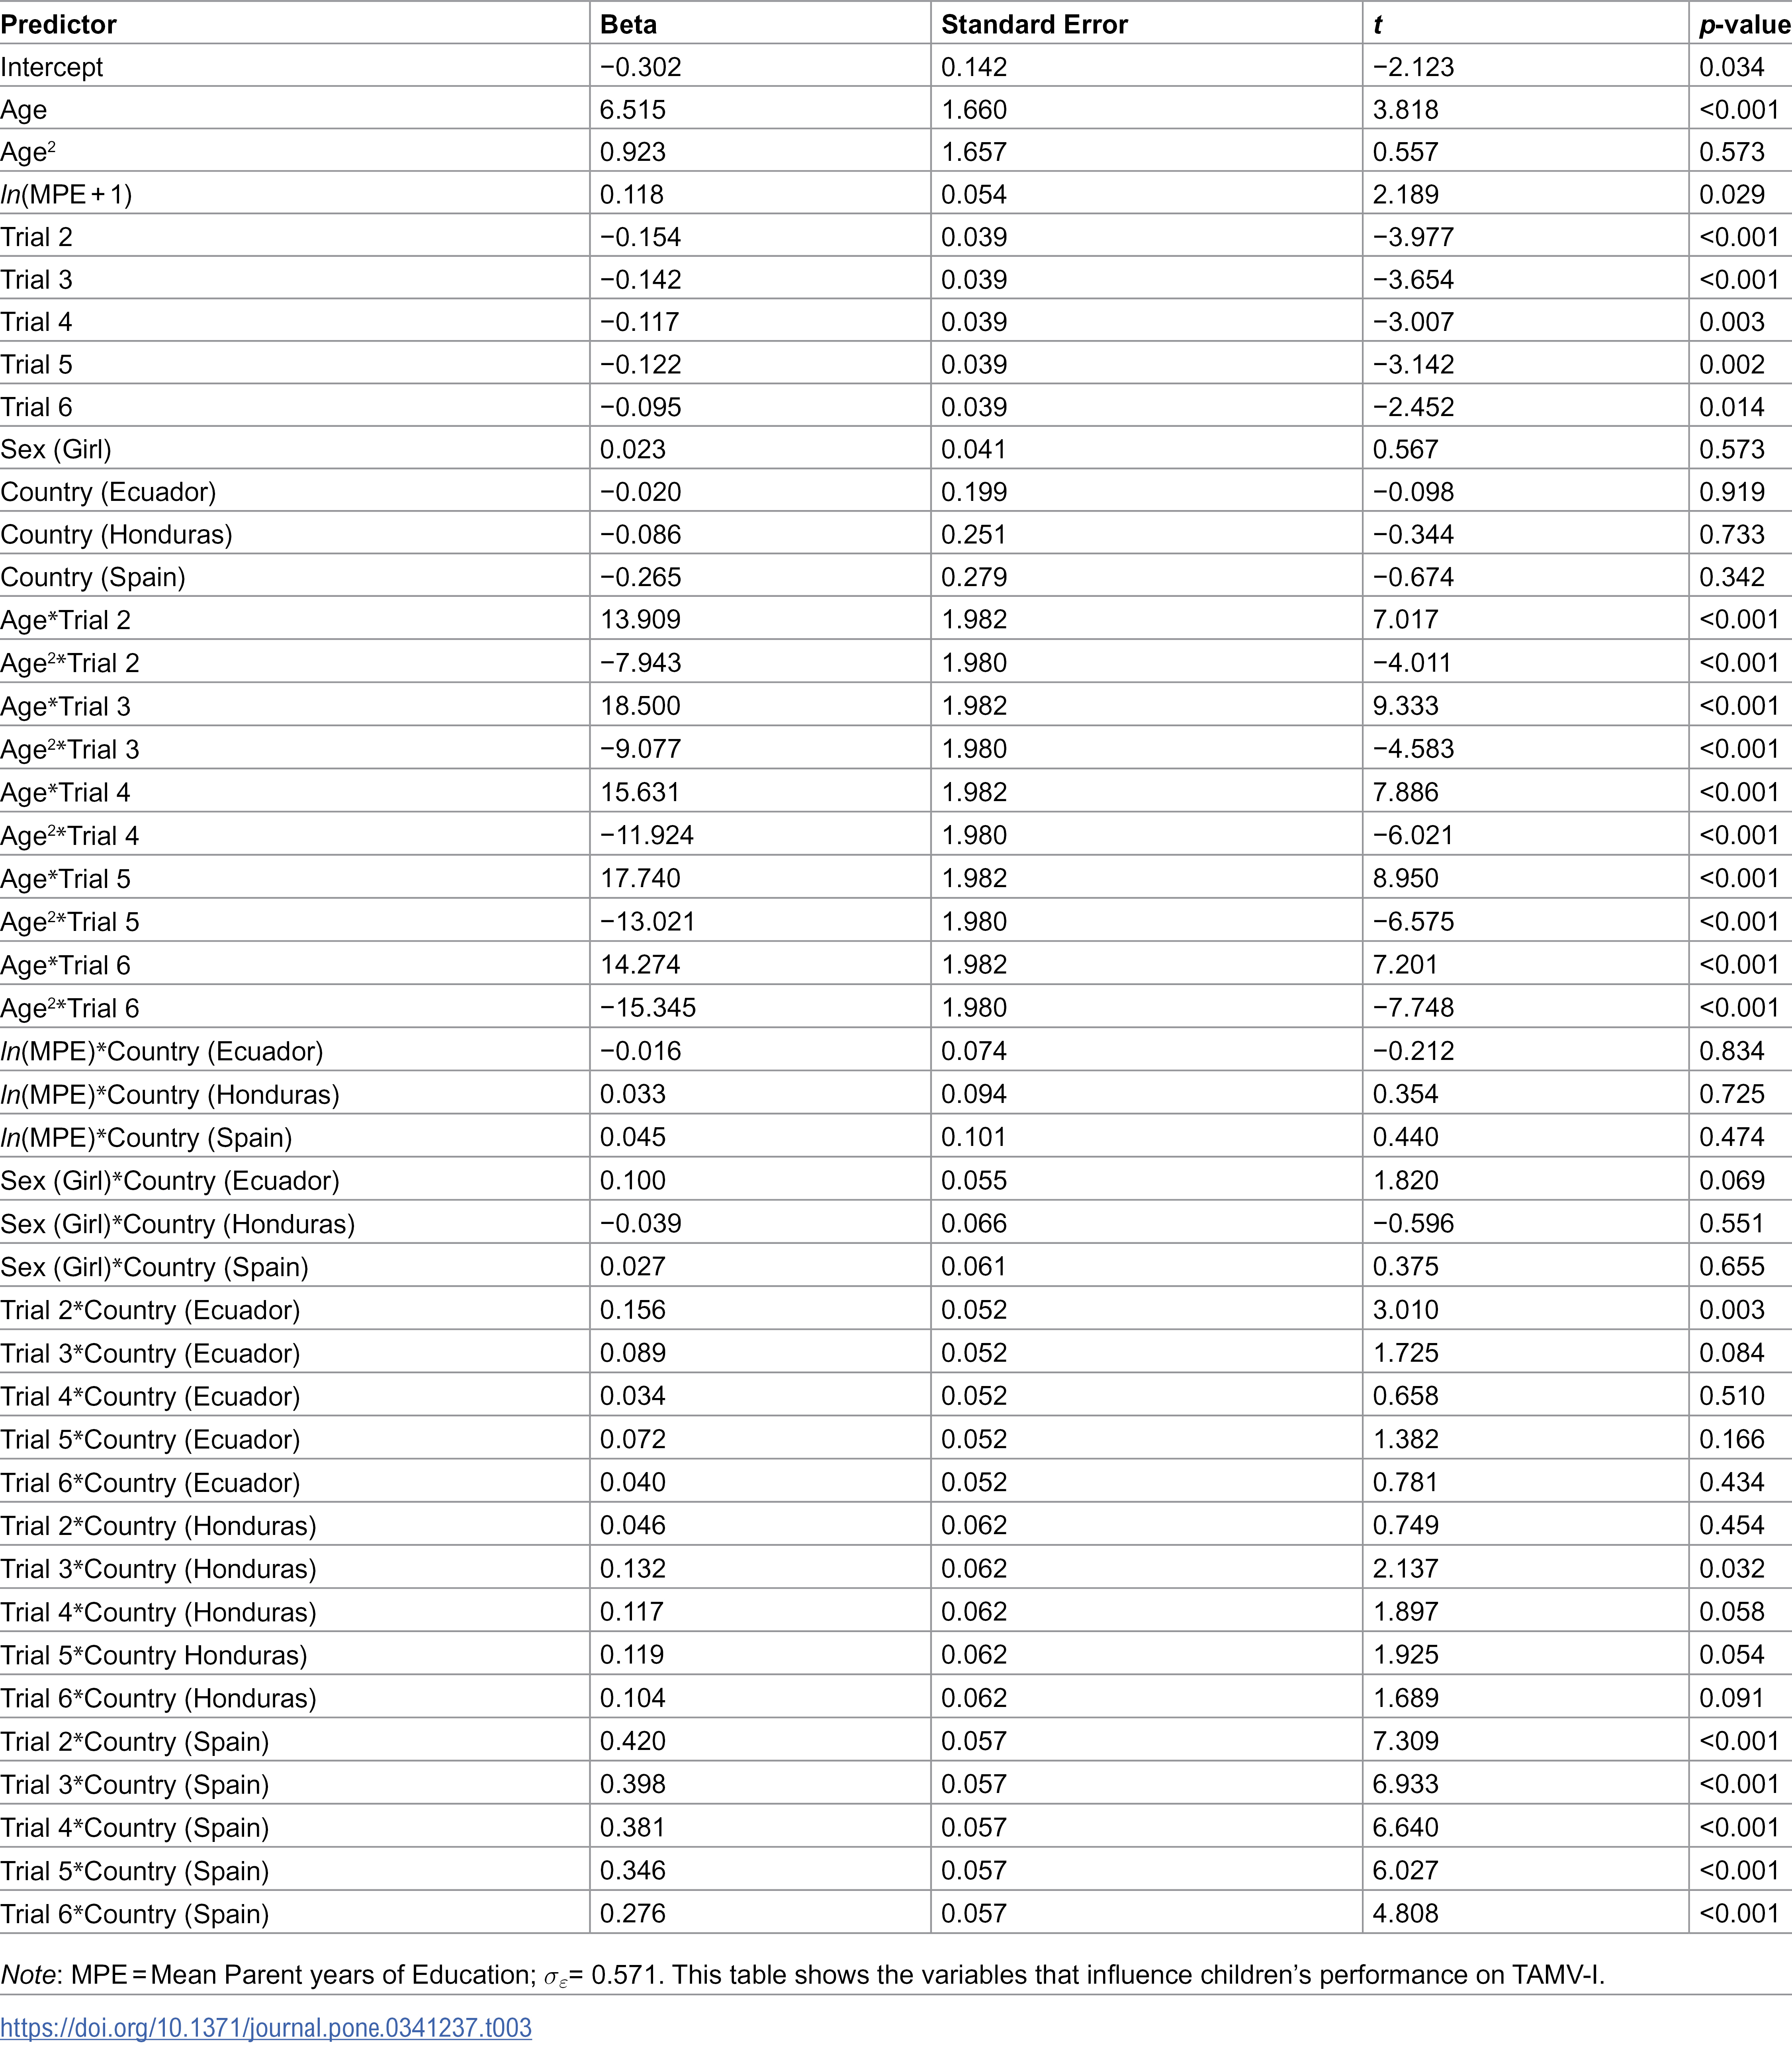
\includegraphics[width=0.45\linewidth]{journal.pone.0341237.t003}
			\caption{}
			\label{fig:journale}
		\end{figure}
\end{frame}

\begin{frame}{Efecto de las variables demográficas en la habilidad II}
	\vspace{-0.5cm}
	\begin{figure}
		\centering
		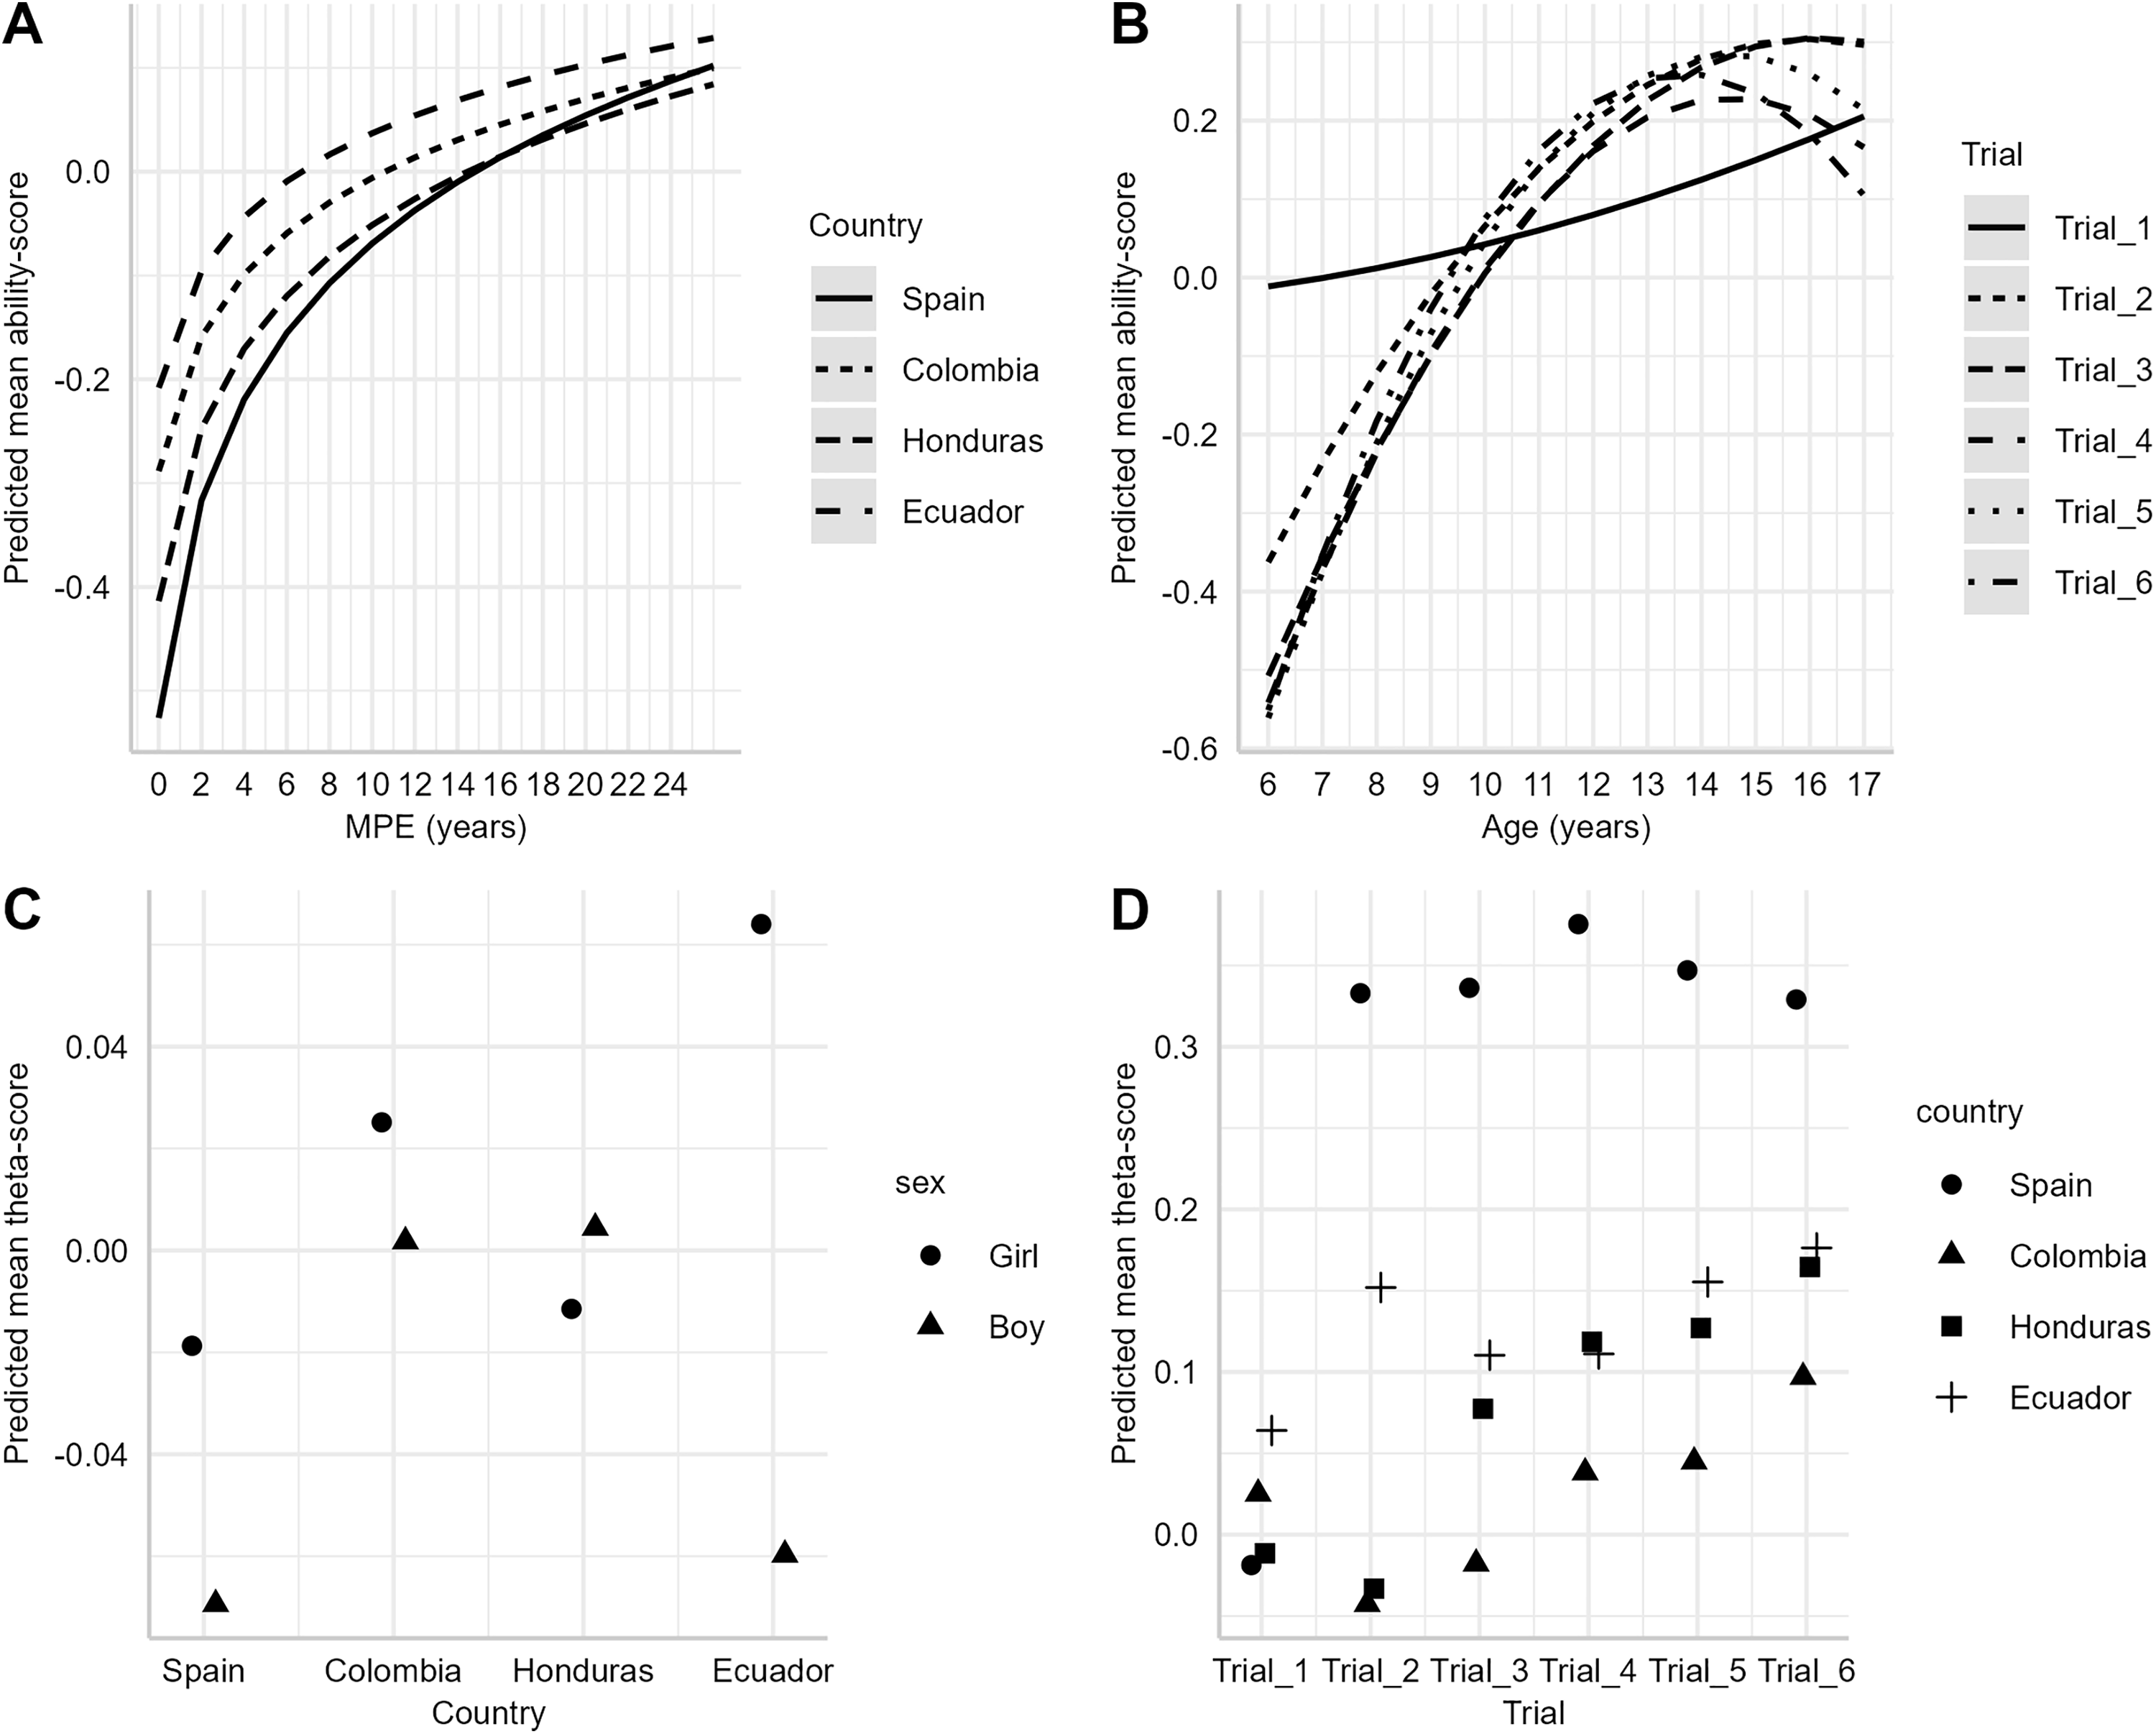
\includegraphics[width=0.61\linewidth]{journal.pone.0341237.g003}
		\caption{}
		\label{fig:journalf}
	\end{figure}
	
\end{frame}

\subsection{Aplicación de datos normativos}

\begin{frame}{Aplicación de datos normativos}
		\vspace{-0.5cm}
		\begin{columns}[T]
			
			\begin{column}{0.5\textwidth}
				\centering
				\textbf{Calculadora de datos normativos}
				
%				\vspace{0.1cm}
				
				\begin{figure}
					\centering
					
\includegraphics[width=0.8\linewidth]{calculadora}
					\label{fig:calculadora}
				\end{figure}
				
				
			\end{column}
			
			\begin{column}{0.5\textwidth}
				\centering
				\textbf{Códigos reproducibles}
				
%				\vspace{0.1cm}
				
				\begin{figure}
					\centering
					
\includegraphics[width=0.8\linewidth]{reproducible}
					\label{fig:reproducible}
				\end{figure}
				
				
			\end{column}
			
		\end{columns}
		
  \end{frame}

\section{Conclusiones}

\begin{frame}{Conclusiones}
	
	\begin{enumerate}
		\item Se desarrollaron datos normativos utilizando IRT y modelos lineales mixtos (LMM).
		
		\vspace{0.6cm}
		
		\item El modelo 2PL mostró un mejor ajuste que el modelo de Rasch según la razón de verosimilitud. El BIC favorece a 2PL solo en los ensayos 1–3, en los ensayos 4, 5 y 6 Rasch tiene menor BIC.
		
		\vspace{0.6cm}
		
		\item Edad, Ensayos 2-6, $\ln MPE$, Edad $\times$ Ensayos, Edad$^2$ $\times$ Ensayos y País $\times$ Ensayos, sobre España  influyen significativamente en el desempeño.
		
		\vspace{0.6cm}
		
		\item Se desarrolló una herramienta en línea que facilita el cálculo e interpretación de puntuaciones normativas.
		
%		\vspace{0.2cm}
%		
%		\item Los datos están disponibles en: \href{https://zenodo.org/records/18176818}{https://zenodo.org/records/18176818}
		
	\end{enumerate}
\end{frame}

\section{Referencias}

\begin{frame}[allowframebreaks]{Referencias}
	\scriptsize
	\bibliographystyle{apalike}
	\bibliography{biblio_intro}
\end{frame}

\begin{frame}
	Este trabajo fue publicado en \texttt{Plos One}\\	
	\bigskip
	Fuentes Mendoza EM, Olabarrieta-Landa L, Rodríguez-Lorenzana A, Mascialino G, Vergara-Moragues E, et al. (2026) Normative Data for Learning and Memory Test (TAMV-I) in Latin American and Spanish Children: An item response theory and linear mixed models approach. \textit{PLOS ONE} 21(2): e0341237. \href{https://doi.org/10.1371/journal.pone.0341237}{https://doi.org/10.1371/journal.pone.0341237}
\end{frame}

\setbeamertemplate{background canvas}{
	
\includegraphics[width=\paperwidth, height=\paperheight]{front.jpg}
}


\begin{frame}{}
	\vspace{2cm}
	\centering
	\textcolor{white}{{\Huge  \textbf{¡Gracias!}}}\\
	\textcolor{white}{{\Huge  \textbf{¿Preguntas?}}}
\end{frame}

\end{document}
